\clearpage
\section{Unconstrained Optimization}
The code solving the unconstrained optimization problems can be found in the software package submitted.
There are different search algorithms used to find the solutions to unconstrained nonlinear problems briefly explained below. 
\textbf{\subsection{Algorithms To Solve Unconstrained Nonlinear Programming Problems}} 
There are different algorithms that can solve general unconstrained nonlinear programming problems. These include:
\begin{enumerate}
    \item Steepest Descent search algorithm
    \item Secant Algorithm
    \item Conjugate gradient Method
\end{enumerate}
\subsubsection{Steepest Descent Algorithm}
 Steepest Descent is a first-order iterative optimization algorithm to find a local minimum of a differentiable function. The idea is to take repeated steps in the opposite direction of the gradient of the function at the current point, because this is the direction of steepest descent. Overview of the Steepest Descent Algorithm is provided below: 
\SetKwInOut{Input}{Input}
\SetKwInOut{Output}{Output\,}
\SetAlgoLined
\DontPrintSemicolon
\begin{algorithm}[H]
   \textbf{Choose $x_{0}$ \in \mathbb{R}^{n}. Set\hspace{2mm}i = 0}: \newline
   \textbf{Iteration j: } \\
   (1) : Stop \hspace{2mm} if \hspace{2mm} $\nabla V (x_{j})$ = 0 as then $x_{j}$ satisfies a necessary condition for a local minimizer. \\
   (2) : Set $s_{j}$ := -$\nabla V(x_{j})$ \\
   (3) : Choose a scalar $\omega_{j} > 0$, so $V(x_{j} + \omega_{j}s_{j})$ is less than $V(x_{j})$, typically $\omega_{j}$ is chosen to minimize $V(x_{j} + \omega s_{j})$ with $\omega \in \mathbb{R}$\\
   (4) : Set j = j+1 and return to first step.\\
  \caption{\textsc{Steepest Descent Algorithm}}
\end{algorithm}
\subsubsection{Secant Algorithm}
The secant method is a root-finding algorithm that uses a succession of roots of secant lines to better approximate a root of a function f. The secant method is a finite-difference approximation of Newton's method. It is also known as a quasi-newton method. Overview of the Secant Algorithm is provided below: 
\SetKwInOut{Input}{Input}
\SetKwInOut{Output}{Output\,}
\SetAlgoLined
\DontPrintSemicolon
\begin{algorithm}[H]
   \textbf{Choose $x_{0}$ \in \mathbb{R}^{n}.}: \newline
   \textbf{Symmetric positive definite $H_{0} \in \mathbb{R}^{n x n}$, $H_{0}$ is an estimate of unknown $C^{-1}$}\newline 
   Set \hspace{2mm} j := 0 \\
   \textbf{Iteration} \hspace{2mm} j: \\
   (1) : Set \hspace{2mm} $s_{j}$ = -$H_{j}\nabla V(x_{j})$ (pseudo-Newton search direction). \\
   (2) : Choose $\omega_{j} \geq$ 0 so $V(x_{j} + \omega_{j}s_{j})$ less than $V(x_{j})$ \\
   (3) : Set $x_{j+1}$ = $x_{j} + \omega_{j}s_{j}$ \\
   (4) : Stop if $||\nabla V(x_{j+1})||$ less than $\epsilon$ = small \\
   (5) : $\triangle x_{j}$ = $x_{j+1} - x_{j}$, $\triangle g_{j}$ = $\nabla V(x_{j+1}) - \nabla V(x_{j})$ \\
   (6) : Choose symmetric positive definite $H_{j+1} \in \mathbb{R}^{nxn}$ so \\
   $H_{j+1} \cong C^{-1}$ - improved \\
   (7) : Set $j = j+1$ and return to (1) \\
  \caption{\textsc{Secant Algorithm}}
\end{algorithm}
The most famous way to choose $H_{j}$ is the David Fletcher Powell Algorithm. 

\subsubsection{Conjugate Gradient Method}
Conjugate direction methods can be regarded as being between the method of steepest descent (first-order method that uses gradient) and Newton’s method (second-order method that uses Hessian as well). It accelerates the convergence rate of steepest descent while avoiding the high computational cost of Newton’s method. Overview of the Conjugate Gradient Method is provided below:   
\SetKwInOut{Input}{Input}
\SetKwInOut{Output}{Output\,}
\SetAlgoLined
\DontPrintSemicolon
\begin{algorithm}[H]
   \textbf{Choose $x_{0}$ \in \mathbb{R}^{n}}: \newline
   Set\hspace{2mm} $s_{0}$ = -$\nabla V(x_{0}), j = 0$ \newline 
   (1) : Stop if $||V(x_{j})||$ is less than $\epsilon$ as then $x_{j} \cong x$ \\
   (2) : Choose $\omega_{j} \in$ arg min $V(x_{j} + \omega s_{j})$ \\
   $x_{j+1} = x_{j} + \omega_{j}s_{j}$\\
   (3) : Set $\beta_{j+1} = \frac{[\nabla V(x_{j+1}) - \nabla V(x_{j})]^{T}\nabla V(x_{j+1})}{||\nabla V(x_{j})||^{2}} \in \mathbb{R}$\\
   $s_{j+1} = \nabla V(x_{j+1}) + \beta_{j+1}s_{j}$\\
   the term $\beta_{j+1}s_{j}$ makes the conjugate gradient different from the steepest descent. \\
   $j = j + 1$ and return to (1) \\
  \caption{\textsc{Conjugate Gradient Method}}
\end{algorithm}

\subsection{Quadratic Optimization Problem}
The objective is to minimize the following cost function:
\begin{align}
& \mbox{(A)} : \ \ V(x) = 5+ \left[ \begin{array}{cccccc} 1 & 4 & 5 & 4 & 2 & 1 \end{array} \right] x + x^T \left[ \begin{array}{cccccc}  9 & 1 & 7 & 5 & 4 & 7 \\
1 & 11 & 4 & 2 & 7 & 5 \\ 7 & 4 & 13 & 5 & 0 & 7 \\ 5 & 2 & 5 & 17 & 1  & 9 \\
4 & 7 & 0 & 1 & 21 & 15 \\ 7 & 5 & 7 & 9 & 15 & 27 \end{array} \right] x ; \ \ x \in \mathbb{R}^6 \nonumber \\
\end{align}
This is an unconstrained quadratic optimization problem of the form:
\begin{align}
    V(x) = a + b^{T}x + \frac{1}{2}x^{T}Cx
\end{align},
where 
\begin{align}
    V \in \mathbb{R}, \hspace{2mm} a \in \mathbb{R}, \hspace{2mm} b \in \mathbb{R}^{n},\hspace{2mm} C \in \mathbb{R}^{nxn} \hspace{2mm} and \hspace{2mm} C^{T} = C  \hspace{2mm}& \hspace{2mm} C > 0
\end{align}
C is a positive definite symettric matrix.
This can be solved using the standard quadractic direct solution: 
\begin{align}
    x = -C^{-1}b
\end{align}
or using search algorithms: 
\begin{itemize}
    \item Steepest descent algorithms 
    \item Secant algorithms
    \item Conjugate gradient method 
\end{itemize}
\subsubsection{Solutions to Quadratic problem using our python programs and matlab benchmark \textit{quadprog} function: }
All 4 algorithms converged to the same minimal solution for $x$ with a tolerance set to be $tol =1e-8$ and the same initial value of all column vector of zeros. The gradient loss of the secant algorithm converged to a minimum fastest of our Python-implemented sub-programs as it requires one function evaluation per iteration, following the initial step and it does not require use of the derivative of the function $V(x)$,
while the steepest descent took longest to approach a minimum as it requires to constantly calculate the gradient derivative ($\nabla V(x)$) at every iteration step which is computationally expensive as can be seen in Figure 1. The matlab program used the algorithm \textit{ interior point convex} and quickly found a solution in 1 iteration. \newline All solutions correspond to the standard quadratic solution: 
\begin{align}
    x = -C^{-1}*b = \begin{bmatrix}
     0.3366 \\
    0.0560 \\
   -0.4300 \\
   -0.1920 \\
   -0.2713 \\ 
    0.2101 \\
    \end{bmatrix} 
\end{align}
\begin{table}[htbp]
\begin{center}
\begin{tabular}{|c|c|c|c|c|}
\hline
 & \textbf{Steepest Descent} & \textbf{Secant} &\textbf{Conjugate Method} &\textbf{\textit{quadprog}}\\
\hline
Iterations & 107 & 14 &37& 1 \\
\hline
$x$ & 
\begin{bmatrix}
0.3365 \\
 0.0560 \\
 -0.4300   \\
 -0.1919  \\
 -0.2713 \\
 0.2100 \\
\end{bmatrix}
&\begin{bmatrix}
 0.3365 \\
 0.05604  \\ 
 -0.4300 \\
 -0.1919 \\
 -0.2713 \\
 0.2100 \\
\end{bmatrix} & \begin{bmatrix}
0.3365 \\
0.05604\\
-0.4300 \\
-0.1919 \\
-0.2713 \\ 
0.2101\\
\end{bmatrix} &\begin{bmatrix}
     0.3366 \\
    0.0560 \\
   -0.4300 \\
   -0.1920 \\
   -0.2713 \\
    0.2101 \\
\end{bmatrix} \\
\hline 
\end{tabular}
\label{table:results}
\caption{Algorithm Performance}
\end{center}
\end{table}

\begin{figure}[h!]
\begin{subfigure}[t]{0.6\textwidth}
\centering
    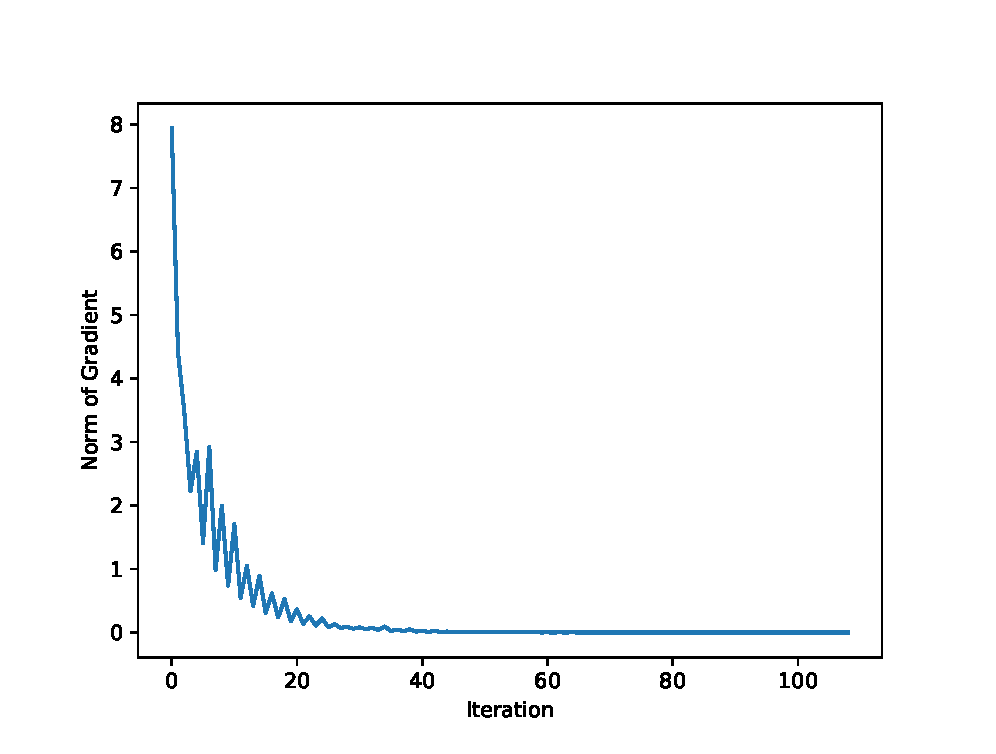
\includegraphics[width=\textwidth]{images/python/sd-pA.eps}
\caption{}
\end{subfigure}
\hfill 
\begin{subfigure}[t]{0.6\textwidth}
\centering
    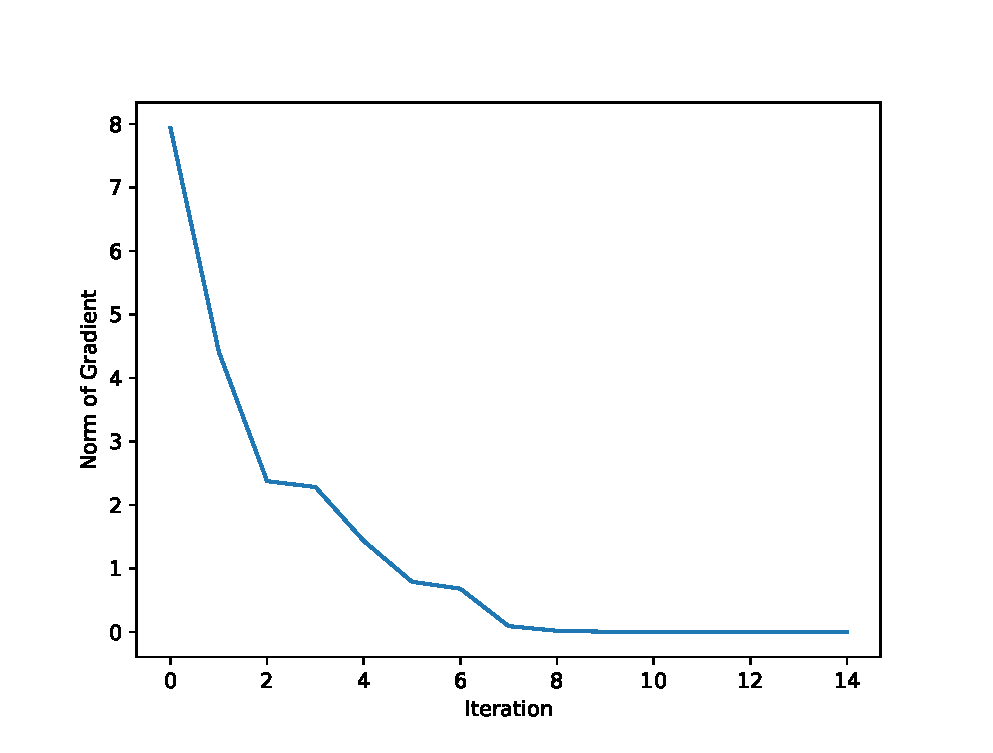
\includegraphics[width=\textwidth]{images/python/sec-pA.eps}
    \caption{}
\end{subfigure}
\hfill
\begin{subfigure}[t]{0.6\textwidth}
\centering
    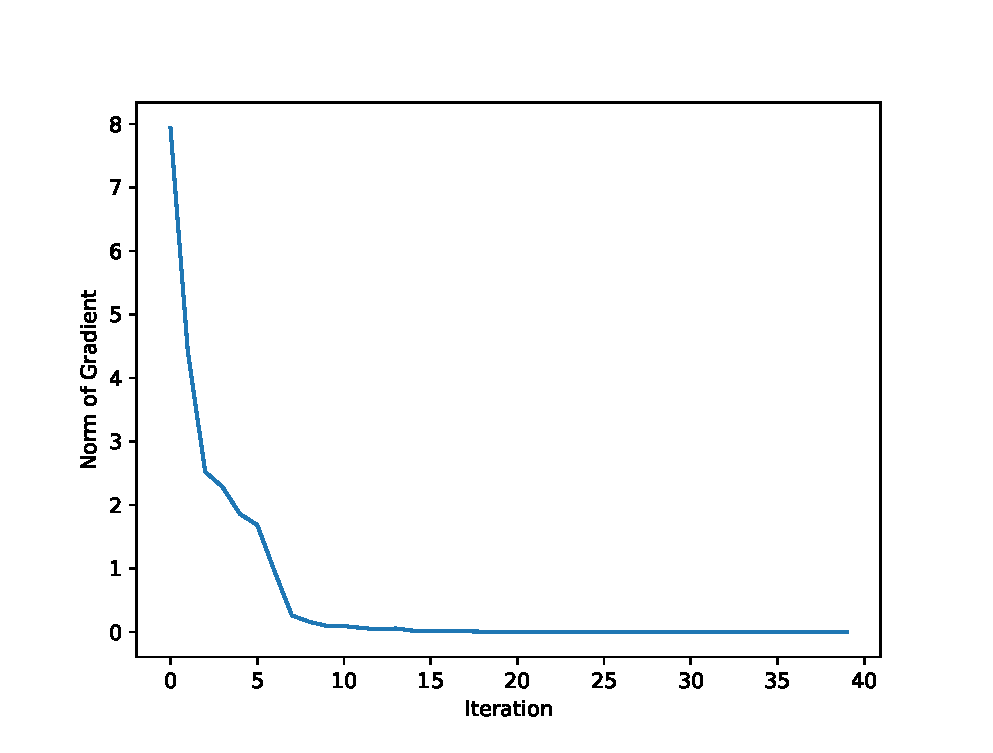
\includegraphics[width=\textwidth]{images/python/cg-pA.eps}
    \caption{}
\end{subfigure}
\caption{(a): Steepest descent, (b): Secant method, (c): Conjugate gradient}
\end{figure}
\clearpage
\subsection{Nonlinear Optimization problem}
The objective is to minimize the following cost function:
\begin{align}
\mbox{(B)} : \ \ V(x) = - \frac{\sqrt{(x_1^2 +1)(2x_2^2 + 1)}}{x_1^2 + x_2^2 + 0.5}; \ \  x \in \mathbb{R}^2 \nonumber \\
\end{align}
This is an unconstrained nonlinear optimization problem of the form:
\begin{align}
    V(x) = f(x)
\end{align}
where 
\begin{align}
    V \in \mathbb{R}
\end{align}
This can be solved using search algorithms: 
\begin{itemize}
    \item Steepest descent algorithms 
    \item Secant algorithms
    \item Conjugate gradient method 
\end{itemize}
\subsubsection{Solutions to unconstrained nonlinear problem using our python programs and matlab benchmark \textit{fminunc} function: }
All four algorithms converged to very close local minimal solutions for $x$ with a tolerance set to $tol =1e-8$ and the same initial value of the column vector of $[-1,1]^{T}$ as confirmed in the contour plot in figure 3. The gradient loss of the secant, conjugate and steepest descent algorithm of our Python-implemented sub-programs converged to a minimum at close to 6 iterations while the matlab implementation used the quasi newton method approached the minimum at 5 iterations.
The contour plot of the function $V(x)$ and the minimum solutions of $x$ derived from the 4 algorithms showed that the lowest value of the objective function for the 4 algorithms exists close to the local minima of the function.
\begin{table}[htbp]
\centering
\begin{center}
\begin{tabular}{|c|c|c|c|c|}
\hline
 & \textbf{Steepest Descent} & \textbf{Secant} &\textbf{Conjugate Method} &\textbf{\textit{Matlab}}\\
\hline
Iterations & 6 & 7 &7& 5 \\
\hline
$x$ & 
\begin{bmatrix}
-4.2345e-09 \\
-5.3553e-09 \\
\end{bmatrix}
&\begin{bmatrix}
 -2.8775e-09 \\
 -2.8274e-09 \\
\end{bmatrix} & \begin{bmatrix}
 -1.0739e-04 \\
 -6.8937e-05 \\
\end{bmatrix} &\begin{bmatrix}
   8.8494e-09 \\
    -2.6837e-10 \\  
\end{bmatrix} \\
\hline 
\end{tabular}
\label{table:results}
\caption{Algorithm Performance}
\end{center}
\end{table}

\begin{figure}[h!]
\centering
\begin{subfigure}[t]{0.4\textwidth}
\centering
    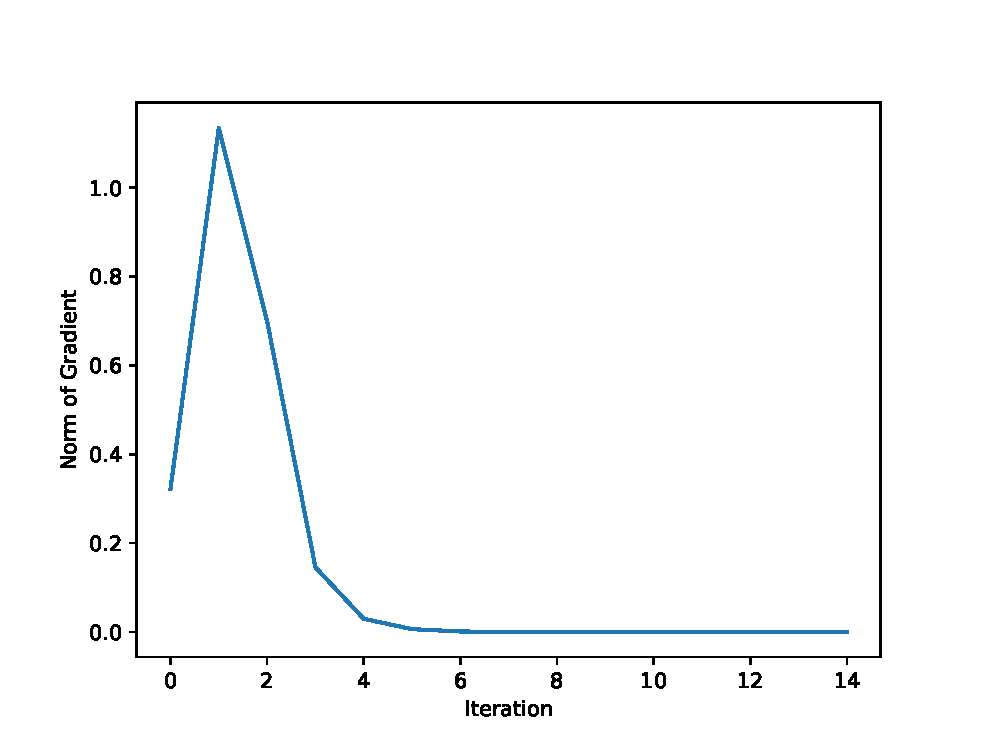
\includegraphics[width=\textwidth]{images/python/sd-pB.eps}
\caption{}
\label{fig:Class distribution}
\end{subfigure}
\hfill 
\begin{subfigure}[t]{0.4\textwidth}
\centering
    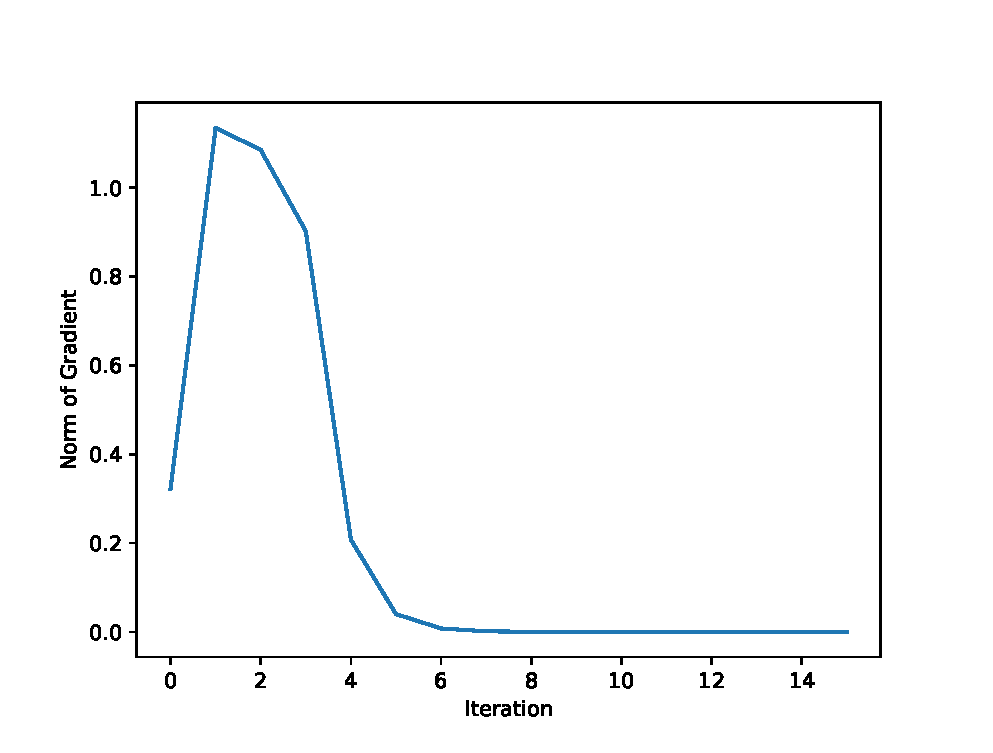
\includegraphics[width=\textwidth]{images/python/sec-pB.eps}
    \caption{}
    \label{fig:TSNE}
\end{subfigure}
\hfill
\begin{subfigure}[t]{0.4\textwidth}
\centering
    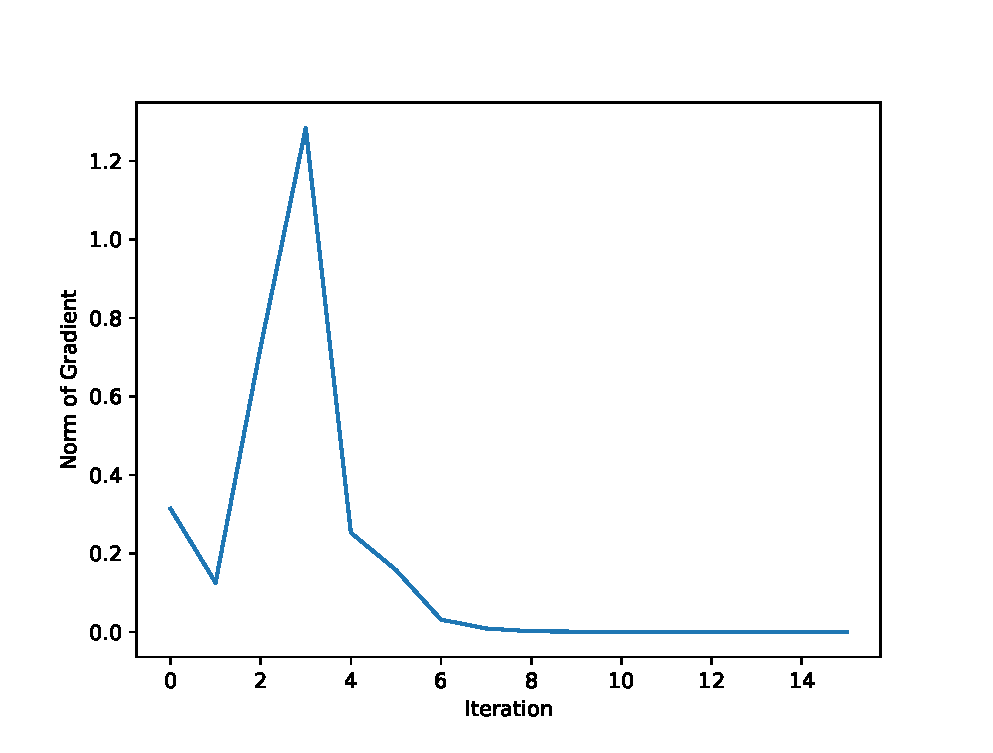
\includegraphics[width=\textwidth]{images/python/cg-pB.eps}
    \caption{}
    \label{fig:TSNE}
\end{subfigure}
\hfill
\begin{subfigure}[t]{0.4\textwidth}
\centering
    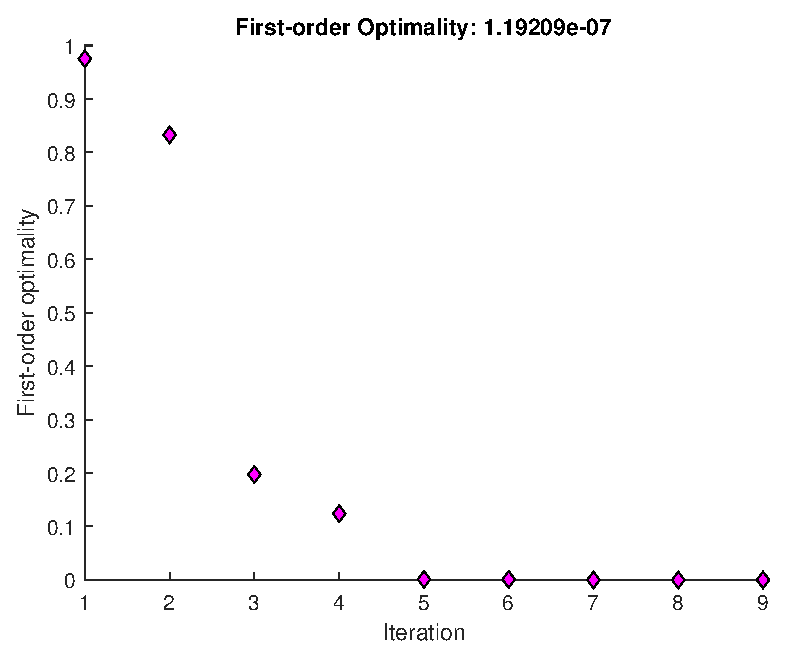
\includegraphics[width=\textwidth]{images/matlab/1b_loss.eps}
    \caption{}
    \label{fig:TSNE}
\end{subfigure}
\caption{(a): Steepest descent, (b): Secant method, (c): Conjugate gradient, (d): Matlab: \textit{fminunc - quasi-newton method}}
\end{figure}
\begin{figure}
    \centering
    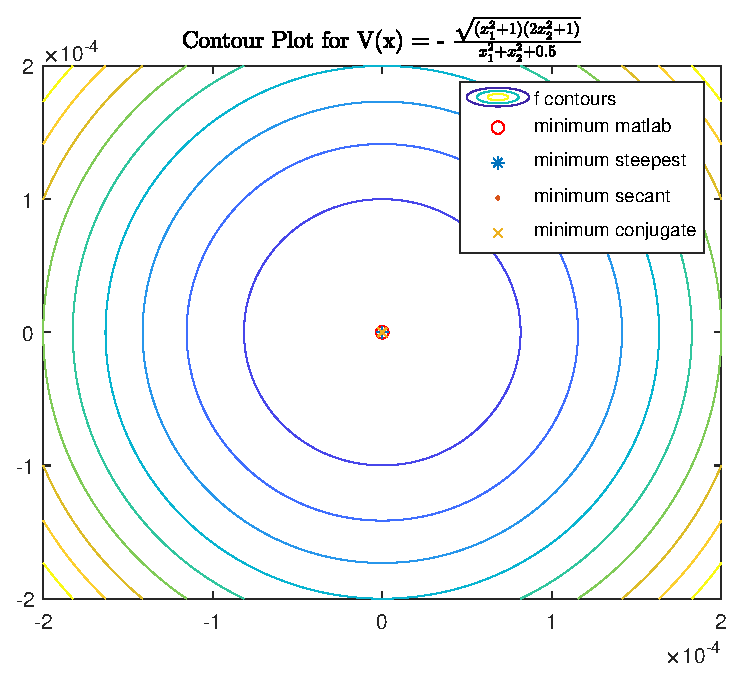
\includegraphics[width=0.4\textwidth]{images/matlab/matlab_1b.eps}
    \caption{Contour Plot for $V(x) = - \frac{\sqrt{(x_1^2 +1)(2x_2^2 + 1)}}{x_1^2 + x_2^2 + 0.5}$ }
\end{figure}
\clearpage
\subsection{Nonlinear Optimization problem}
The objective is to minimize the following cost function:
\begin{align}
& \mbox{(C)}: \ \  V(x) = 1 + \left[ \begin{array}{cc} 1 & 2 \end{array} \right] x + \frac{1}{2} x^T \left[ \begin{array}{cc} 12 & 3 \\ 3 & 10 \end{array} \right] x  \\
& \hspace{2cm} + 10 \mbox{ln}(1+ x_1^4) \mbox{sin}(100x_1)+ 10 \mbox{ln}(1+x_2^4) \mbox{cos}(100x_2)  ; \ \  x \in \mathbb{R}^2  \nonumber
\end{align}
This is an unconstrained nonlinear optimization problem of the form:
\begin{align}
    V(x) = f(x)
\end{align}
where 
\begin{align}
    V \in \mathbb{R}
\end{align}
This can be solved using search algorithms: 
\begin{itemize}
    \item Steepest descent algorithms: 
    \item Secant algorithms: 
    \item Conjugate gradient method: 
\end{itemize}
\subsubsection{Solutions to unconstrained nonlinear problem using our python programs and matlab benchmark \textit{fminunc} function: }
All 4 algorithms converged to very close local minimal solutions for $x$ with a tolerance set to $tol =1e-4$ and the same initial value of column vector of $[0,0]^{T}$ as confirmed in the contour plot in figure 5. The gradient loss of the secant and algorithm converged to a minimum fastest of our Python-implemented subprograms while the conjugate gradient took longest to approach a minimum as can be seen in Figure 4. The Matlab program used the \textit{quasi newton} algorithm and quickly found a solution in 5 iterations.
The contour plot of the function $V(x)$ and the minimum solutions of $x$ derived from the 4 algorithms showed that 
\begin{table}[htbp]
\centering
\begin{center}
\begin{tabular}{|c|c|c|c|c|}
\hline
 & \textbf{Steepest Descent} & \textbf{Secant} &\textbf{Conjugate Method} &\textbf{\textit{Matlab}}\\
\hline
Iterations & 7 & 7 &8& 4 \\
\hline
$x$ & 
\begin{bmatrix}
-0.0177 \\
-0.0958  \\
\end{bmatrix}
&\begin{bmatrix}
 -0.0177 \\
 -0.0954\\
\end{bmatrix} & \begin{bmatrix}
 -0.01772 \\
 -0.0957 \\
\end{bmatrix} &\begin{bmatrix}
   0.080 \\
   -0.6607 \\
\end{bmatrix} \\
\hline 
\end{tabular}
\label{table:results}
\caption{Algorithm Performance}
\end{center}
\end{table}

\begin{figure}[h!]
\centering
\begin{subfigure}[t]{0.4\textwidth}
\centering
    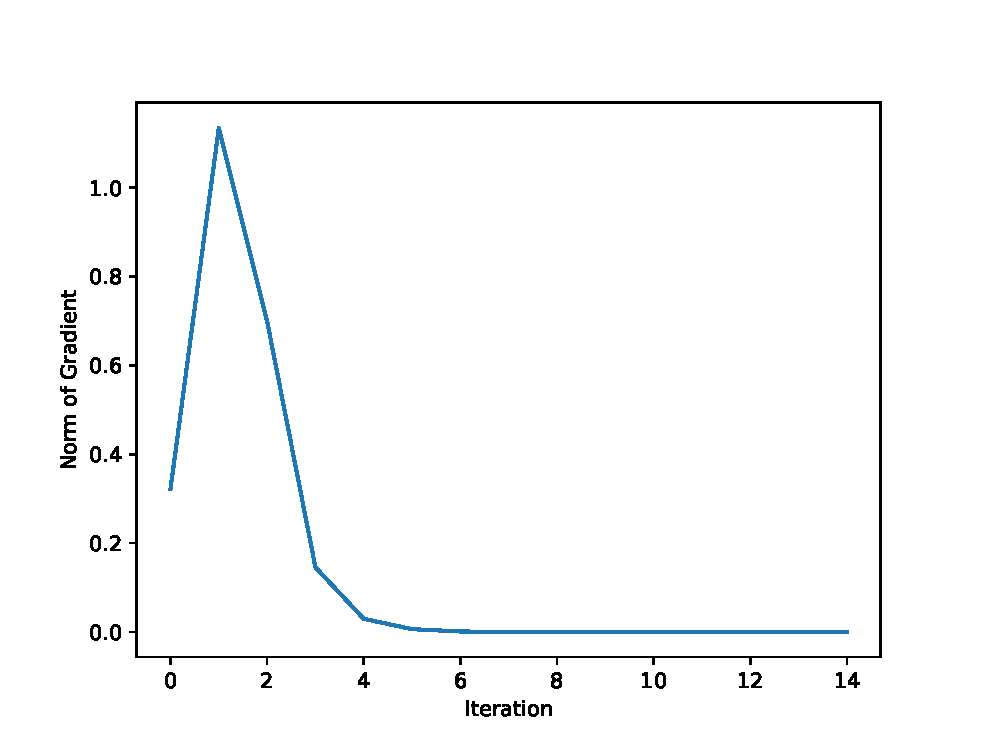
\includegraphics[width=\textwidth]{images/python/sd-pB.eps}
\caption{}
\label{fig:Class distribution}
\end{subfigure}
\hfill 
\begin{subfigure}[t]{0.4\textwidth}
\centering
    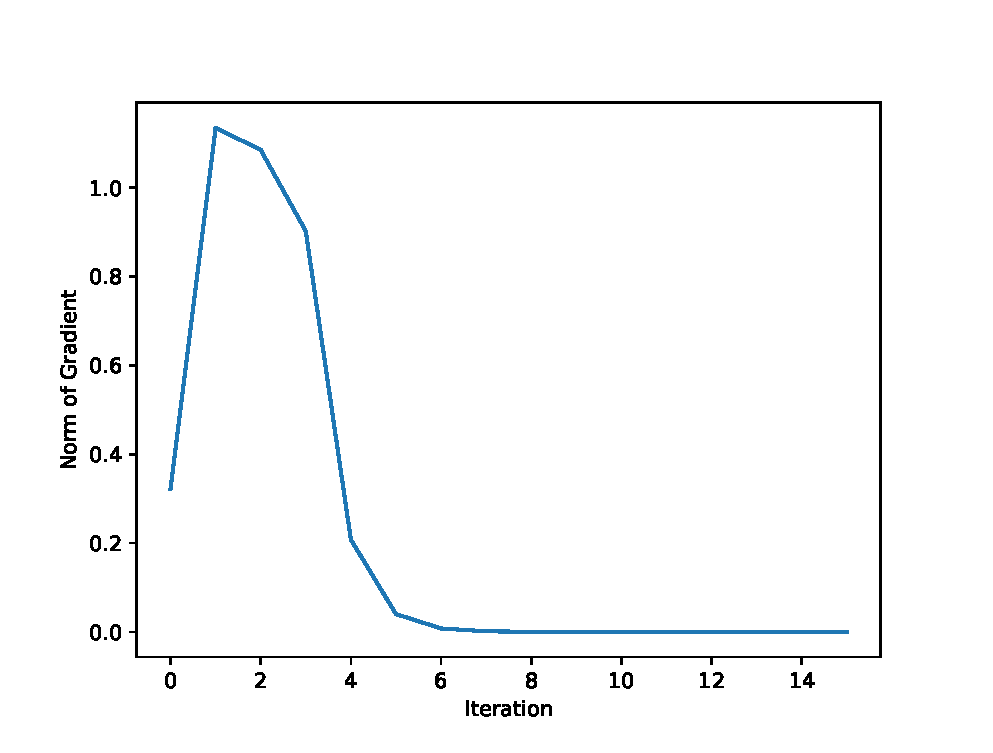
\includegraphics[width=\textwidth]{images/python/sec-pB.eps}
    \caption{}
    \label{fig:TSNE}
\end{subfigure}
\hfill
\begin{subfigure}[t]{0.4\textwidth}
\centering
    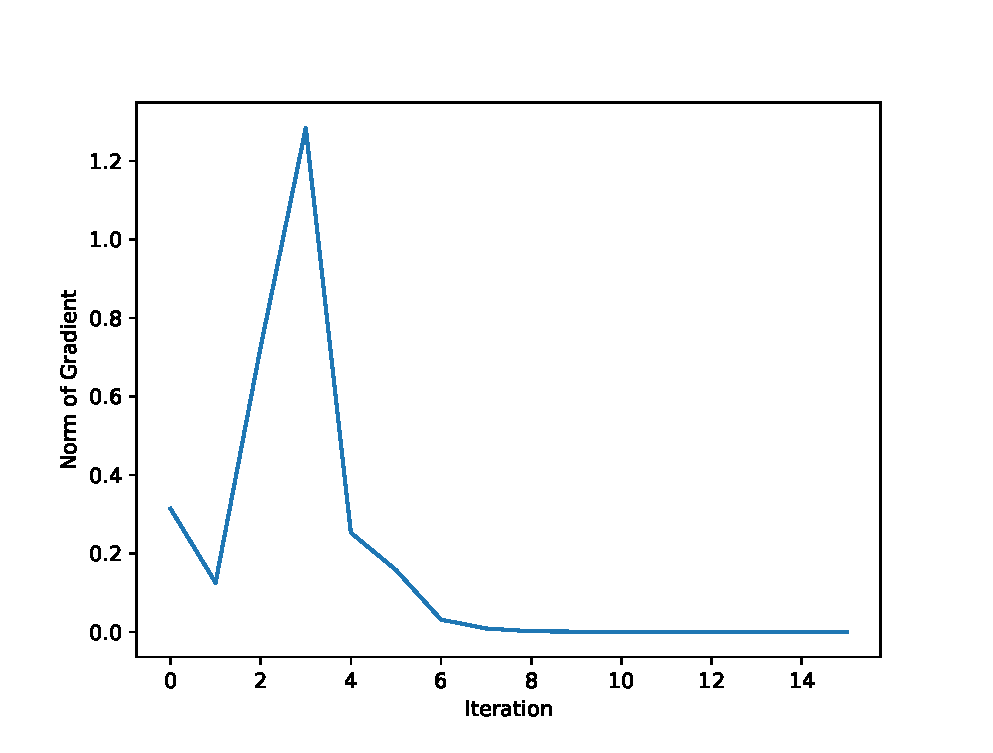
\includegraphics[width=\textwidth]{images/python/cg-pB.eps}
    \caption{}
    \label{fig:TSNE}
\end{subfigure}
\hfill
\begin{subfigure}[t]{0.4\textwidth}
\centering
    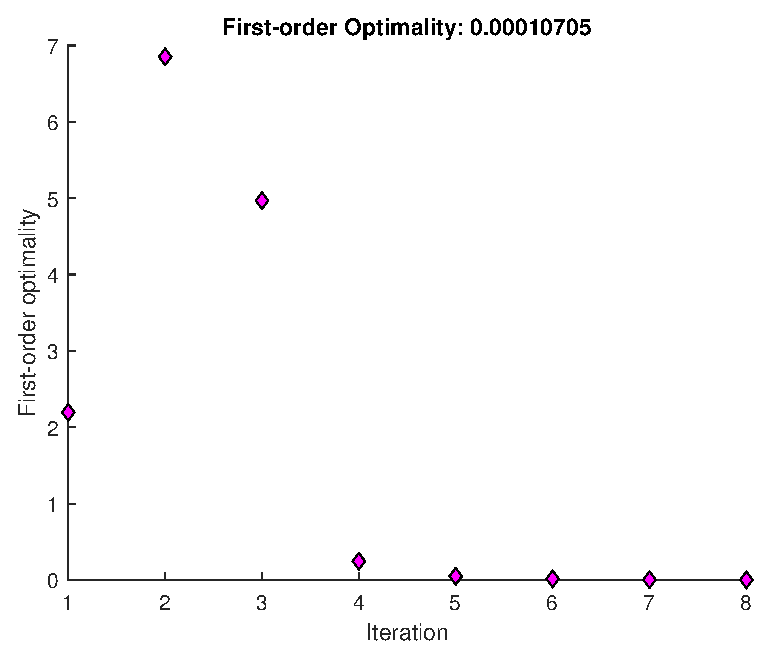
\includegraphics[width=\textwidth]{images/matlab/1c_loss.eps}  
    \caption{}
    \label{fig:TSNE}
\end{subfigure}
\caption{(a): Steepest descent, (b): Secant method, (c): Conjugate gradient, (d): Matlab: \textit{fminunc - quasi-newton method}}
\end{figure}
\begin{figure}
    \centering
    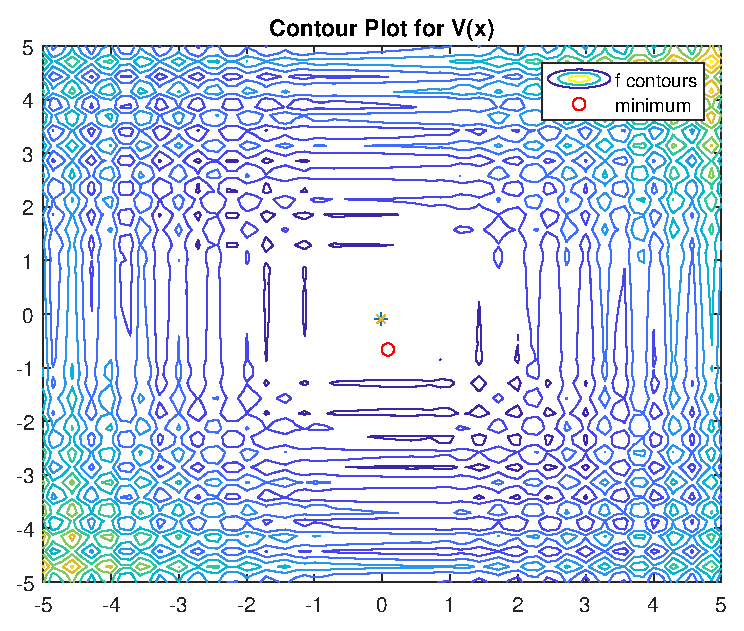
\includegraphics[width=0.4\textwidth]{images/matlab/matlab_1c.eps}
    \caption{Contour Plot for $V(x) = 1 + \left[ \begin{array}{cc} 1 & 2 \end{array} \right] x + \frac{1}{2} x^T \left[ \begin{array}{cc} 12 & 3 \\ 3 & 10 \end{array} \right] x  \hspace{2mm} + 10 \mbox{ln}(1+ x_1^4) \hspace{2mm}\mbox{sin}(100x_1)+ 10 \mbox{ln}(1+x_2^4) \mbox{cos}(100x_2)$}
\end{figure}
